\chapter{Introduction} \label{chapter:intro}

%\hl{INTRODUCTION
%Describe the project idea, its scope, and what are you trying to accomplish. State the most important aspect of the project. This section should contain an overall, high-level description of your project. Include short desrciption of related work and state-of-the art that you cited in references.}

With $23.4\%$ of the daily traffic in North America according to the 2018 \textit{Sandvine} Internet Phenomena Report \cite{sandvinereport}, YouTube is the dominant real-time entertainment service supplier. According to \cite{8976293}, YouTube's popularity has greatly increased over the years. Over a period of four years, YouTube's daily usage by its subscribers has grown from more than $25\%$ in July 2013 to more than $45\%$ in July 2017, as can be seen in the following figure.

\begin{figure}[H]
	\centering
	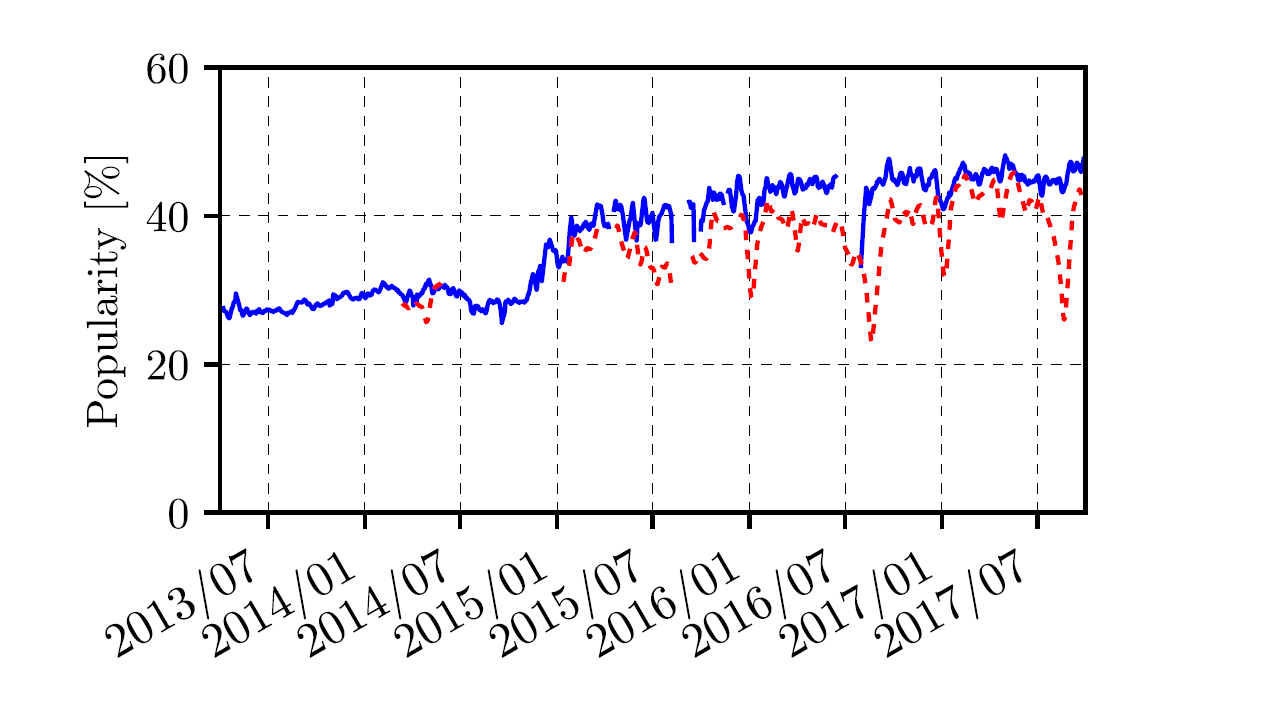
\includegraphics[scale=0.37]{Figures/trevisan2020.png}
	\caption[Popularity of YouTube video streaming]{Popularity of YouTube video streaming from 2013/07 to 2017/07. The blue graph indicates \gls{ADSL} traffic while the red graph represents \gls{FTTH} traffic. Source: \cite{8976293}}
	\label{fig:intro:trevisan}
\end{figure}

In Figure \ref{fig:intro:trevisan}, \gls{ADSL} means Asymmetric Digital Subscriber Line and \gls{FTTH} means Fiber To The Home.

Given YouTube's growing popularity, it is the ideal platform to investigate in this project.

\gls{WiFi} is now available on university campuses, schools, coffee shops, shopping malls, restaurants and even on public transit in some countries. It has become ubiquitous in Canada and it is therefore a good choice of technology to investigate in this report.
 
This project aims to investigate YouTube video streaming over \gls{WiFi} under \gls{QoS} parameters. The discrete network simulator \textit{Riverbed Modeler} will be used to simulate various scenarios and record useful statistics such as throughput and packet delay to see how \gls{WiFi} performs for video streaming.
 
\section{Project objectives, scope and limitations} \label{sec:intro:goals}
The main goal is to simulate YouTube video streaming over \gls{WiFi} with a discrete network simulator. The scope of the project is to simulate network topologies featuring \gls{WiFi} links and applications for YouTube video streaming using Riverbed Modeler. Various scenarios with different types of video streaming at distinct resolutions will be simulated. Phenomena relating to the wireless nature of the technology used will also be investigated, e.g. a client moving with respect to the \gls{WiFi} access point.

The main limitations in this project are imposed by the network simulator used. If a desired feature or module is not available in the chosen network simulator, simulations requiring this feature or module will necessarily be absent in this report.

Before delving into the network topology and simulation scenarios used in this project in Chapter \ref{chapter:simul}, we discuss the background to this project in the following section.

\section{Background} \label{sec:intro:background}
This section provides the background to the project. Video streaming is introduced and discussed in Section \ref{subsec:background:video}. In particular, the specific protocol which YouTube uses, \gls{DASH} is described in this section. This is followed by an overview of \gls{WiFi} technologies employed in this project in Subsection \ref{subsec:background:ieee802}. Subsection \ref{subsec:background:qos} briefly discusses how Quality of Service is measured in this project. The network simulator employed in this work is described in Subsection \ref{subsec:background:riverbed}. A survey of the literature on video streaming simulations using network simulators is presented in Subsection \ref{subsec:background:simu}.  Finally, Subsection \ref{subsec:background:related} provides a review of related projects done previously at SFU.

\subsection{Video streaming} \label{subsec:background:video}
Video streaming allows end-users to play the video while the file contents are being downloaded. YouTube employs \gls{TCP} (Transmission Control Protocol) in the transport layer for video streaming. \cite{rao2011network} In the application layer, YouTube makes use of \gls{DASH}, Dynamic Adaptive Streaming over \gls{HTTP} \cite{ytdash}. Introduced in the open \gls{ISO}/\gls{IEC} 23009-1:2014 Standard \cite{iso2014}, \gls{DASH} is a technique which enables adaptive bitrate streaming over \gls{HTTP}. The latest (revised) version of the Standard is \gls{ISO}/\gls{IEC} 23009-1:2019 \cite{iso2019}. YouTube uses a variant of \gls{DASH} known as \gls{MPEG}-\gls{DASH} \cite{ytdash} (\gls{MPEG}-\gls{DASH} stands for Motion Picture Experts Group - Dynamic Adaptive Streaming over \gls{HTTP} \cite{mpeg}). \gls{DASH} entails encoding chunked media content (e.g. video or audio files) at multiple bit rates and storing them along with a \textit{manifest file} on the server side. The manifest file contains a \gls{URL} for each file chunk encoded at each bit rate, as can be seen in Figure \ref{fig:intro:dash}. The chunks have a duration of 2 to 10 seconds \cite{lederer}.

\begin{figure}[H]
	\centering
	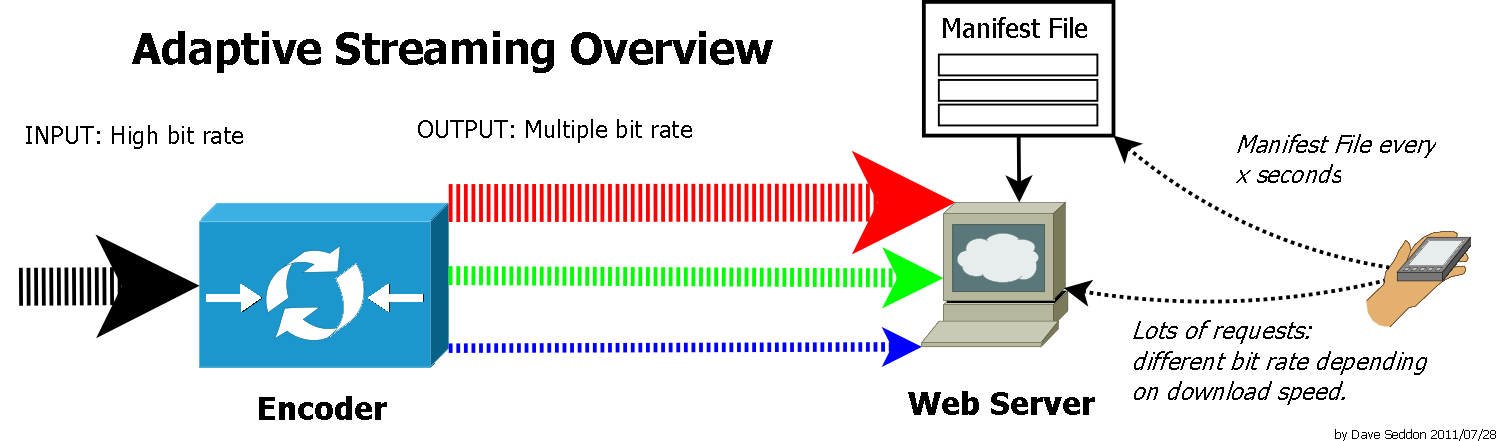
\includegraphics[scale=0.2]{Figures/Adaptivestreami.png}
	\caption[Adaptive Streaming Overview]{Adaptive Streaming Overview \cite{dashimg}. The encoder outputs streams at multiple bit rates which contain chunks of variable length. The client requests chunks from different bit streams according to the currently available bandwidth.}
	\label{fig:intro:dash}
\end{figure}

On the client side, the server-to-client bandwidth and the client's CPU capacity are measured regularly and the quality of the media stream is fine-tuned to the maximum coding rate which can suit these conditions. This implies that the client can choose different coding rates at various points in time according to the available bandwidth at that time, as illustrated in Figure \ref{fig:intro:maza} from \cite{maza2016framework}.
\begin{figure}[H]
	\centering
	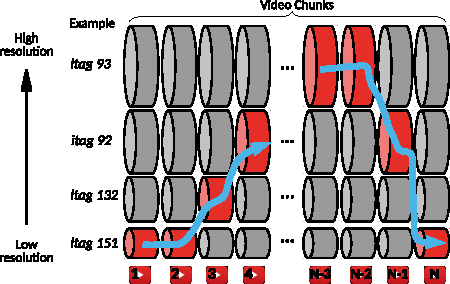
\includegraphics[scale=1]{Figures/mazayt.pdf}
	\caption[YouTube's streaming strategy]{YouTube's streaming strategy \cite{maza2016framework}: over time, the streaming client receives chunks encoded at varying resolutions.}
	\label{fig:intro:maza}		
\end{figure}

\subsection{IEEE 802.11 technologies} \label{subsec:background:ieee802}
\gls{IEEE802} protocols are \gls{WLAN} standards created and curated by the IEEE\footnote{Institute of Electrical and Electronic Engineers. \url{https://www.ieee.org/}} 802.11 Working Group\footnote{\url{http://www.ieee802.org/11/}}.

The first \gls{IEEE802} standard considered in this work is 802.11a which has a maximum theoretical data rate of $54~\textrm{Mbit/s}$. The frequency range is around $5~\mathrm{GHz}$ \cite{banerji2013ieee} which is an unlicensed frequency band. Since the associated wavelength is of the order of $6~\mathrm{cm}$, it is readily absorbed by objects and walls in buildings. On the other hand, 802.11g \gls{WiFi} which operates at $2.4~\mathrm{GHz}$ is less readily absorbed. \gls{WiFi} at $2.4~\mathrm{GHz}$  is also in an unlicensed frequency band. Due to the fact that several devices also operate at $2.4~\mathrm{GHz}$ such as microwave ovens, Bluetooth-enabled devices, cordless phones, baby monitors, car alarms and garage door openers \cite{lifewire}, electromagnetic interference may occur if a \gls{WLAN} operates in the $2.4~\mathrm{GHz}$ frequency band. 802.11g also has a maximum theoretical data rate of $54~\textrm{Mbit/s}$. \cite{banerji2013ieee} These technologies are effectively combined in 802.11n: it operates in both frequency ranges, $2.4~\mathrm{GHz}$ and $5~\mathrm{GHz}$. 802.11n differs in the sense that it may be implemented in \gls{MIMO} (Multiple Input, Multiple Output) systems with multiple transmitting antennas and different modulation schemes. \cite{banerji2013ieee} Furthermore, it has increased the maximum theoretical data rate to $72~\mathrm{Mbit/s}$. Modern devices such as smartphones are now being developed to be dual-band compatible so that they may operate in both frequency bands of 802.11n. Since fewer devices exploit the higher $5~\mathrm{GHz}$ range, this means that a larger number of hosts may be accommodated by a $5~\mathrm{GHz}$ \gls{WLAN}.

\subsection{Quality of Service} \label{subsec:background:qos}
The term `Quality of Service' (\gls{QoS}) is used to quantify the overall performance of a network. It comprises of the following parameters \cite{qos}:
\begin{itemize}
	\item Throughput 
	\item Packet loss
	\item Latency
	\item Jitter
\end{itemize}

%Throughput, measured in bits/second, measures the rate of successful packet delivery over the network.
In this project, we mainly investigated throughput and packet delay (latency).

\subsection{Riverbed Modeler} \label{subsec:background:riverbed}
\textit{Riverbed Modeler} is a modeling and simulation environment which can be used to simulate computer networking scenarios. \cite{riverbed}. It is a proprietary software whose \textit{Academic Edition} used in this course provides a restricted set of functionalities. \textit{Riverbed Modeler} provides a Graphical User Interface which permits the user to create simulations quickly, without having to develop simulation scripts or coding libraries, unlike the open-source discrete event simulator \gls{ns3} \cite{nsnamwiki}. Due to the time-constrained nature of this project, we opted for \textit{Riverbed Modeler Academic Edition version 17.5} over \gls{ns3}.

However, the Academic Edition has some limitations \cite{riverbedrestrictions} which restrict the simulations envisaged in this project:
\begin{itemize}
	\item The Academic Edition software does not allow the user to import capture files/trace files discrete network simulations.\\ This is an issue since we envisaged collecting trace files of video streaming over \gls{WiFi} and \gls{lte} and passing these into our Riverbed Modeler simulations.
%	\item The Academic Edition software does not have a video streaming module. \\
%	This is an issue since we wanted to simulate video streaming. The makeshift solution is to tailor the videoconferencing module to simulate video streaming. 
	\item The Academic Edition software does not support System-In-The-Loop simulations.\\
	We envisaged using our computers connected to \gls{WiFi} networks as systems-in-the-loop in simulations.
\end{itemize}


\subsection{Video streaming simulations with network simulators} \label{subsec:background:simu}
In 2014, Hassan \textit{et al.} reported on real-time video streaming experiments done with the System-In-The-Loop (SITL) module of \gls{OPNET} (the predecessor to Riverbed Modeler) using WiMax in \cite{7016825}. Employing \gls{DASH}, they used video segments of varying duration to investigate the influence on bandwidth utilization and CPU resource utilization at the streaming client.

In 2017, using \gls{OPNET}, Mohamed and Ibrahim simulated video streaming over \gls{lte} featuring \begin{itemize*}
	\item co-channel interference between adjacent cells
	\item jamming by a jammer node to cancel co-channel interference
\end{itemize*} in \cite{8275396} \gls{QoS} parameters such as throughput, jitter and end-to-end delay were recorded. 

\subsection{Related work at SFU} \label{subsec:background:related}
A number of previous projects in this course also focused on video streaming over \gls{WiFi}. They were informative in our investigations.

\begin{itemize}
	\item \textit{Video Streaming over the 802.11g \gls{WLAN} Technologies}, Spring 2011. \cite{xue} \\
	Xue made use of \gls{OPNET} (the original incarnation of \textit{Riverbed Modeler}) to investigate three cases in \cite{xue}:
	\begin{itemize}
		\item a \gls{IEEE802}g \gls{WLAN} simulation with various data rates.
		\item a \gls{IEEE802}g \gls{WLAN} simulation with a faster server.
		\item a \gls{IEEE802}g \gls{WLAN} simulation with a server with more powerful transmit power.
	\end{itemize}
	Metrics such as packet end-to-end delay and throughput were collected and analyzed \cite{xue}.
	\item \textit{Performance Analysis of a Wireless Home Network} \cite{calzada} \\
	Calzada \textit{et al.} used the videoconferencing application of \gls{OPNET} to simulate video streaming, among several other scenarios, such as web browsing and \gls{VoIP} (Voice over Internet Protocol). The delay resulting from these applications were compared in \cite{calzada}.
	\item \textit{Performance Analysis of Video Streaming over \gls{WiFi} and Ethernet}, Spring 2015. \cite{arshit} \\
	Singh and Labayo in \cite{arshit} used \textit{Riverbed Modeler} to run the following scenarios:
	\begin{itemize}
		\item Ethernet with a single host (workstation).
		\item \gls{WLAN} with a single host.
		\item Both Ethernet and \gls{WLAN} with a single host.
		\item Both Ethernet and \gls{WLAN} with two hosts.
	\end{itemize}
	The video conferencing module of \textit{Riverbed Modeler} was used to simulate video streaming \cite{arshit}.
	\item \textit{Video Streaming over \gls{WiFi}}, Spring 2015. \cite{kim} \\
	Kim \textit{et al.} simulated a home network and ran the following scenarios in \textit{Riverbed Modeler}: light browsing, heavy browsing, \gls{VoIP} (Voice over Internet Protocol), and video conferencing of movies' traces to simulate video streaming. \cite{kim} The simulations were adapted to investigate changing data rate, changing the protocol from \gls{IEEE802}a to \gls{IEEE802}g  to \gls{IEEE802}n and finally, varying the distance between the \gls{WiFi} access point and the host. \cite{kim}
	\item \textit{Video Streaming over \gls{WiFi} using Riverbed Modeler}, Spring 2016. \cite{michaelng} \\
	Ng and Weng also simulated a home network and ran two types of scenarios: \begin{itemize}
		\item Light browsing, heavy browsing and video streaming.
		\item Streaming two movies and varying attributes, such as data rate, to the server.
	\end{itemize}
	Metrics such as throughput, delay and jitter were collected and analyzed. \cite{michaelng}
\end{itemize}

%\hl{Explain what we learnt from these and how that guided us in our decisions in the following chapter.}
%\section{Summary} \label{sec:intro:summary}
%
%\hl{summarize what we talked about in here. reminder of what we are trying to accomplish. create the link between this chapter and the next one.}
%

\section{Report overview} \label{sec:overview}
This report is structured as follows:
\begin{itemize}
	\item Chapter \ref{chapter:simul} describes in detail the design and execution of the simulation experiments conducted in this project. Based on the foregoing discussion in the literature review in Section \ref{subsec:background:related}, experiments were designed to best accomplish the objectives of this project using the software tool chosen. Results from the simulations are shown and discussed in depth.
	\item Chapter \ref{chapter:discussion} reviews the experiments in the previous chapter. It outlines how the goals of this project were achieved. Furthermore, Chapter \ref{chapter:discussion} puts forth our recommendations for future work.
	\item Appendix \ref{appendix:a} provides important information which will help the reader to replicate our experiments and to re-create our report from the source files. 
\end{itemize}